\documentclass{article}
\usepackage[margin=1in]{geometry}
\usepackage[linesnumbered,ruled,vlined]{algorithm2e}
\usepackage{amsfonts}
\usepackage{amsmath}
\usepackage{amssymb}
\usepackage{amsthm}
\usepackage{enumitem}
\usepackage{fancyhdr}
\usepackage{hyperref}
\usepackage{minted}
\usepackage{multicol}
\usepackage{pdfpages}
\usepackage{standalone}
\usepackage[many]{tcolorbox}
\usepackage{tikz-cd}
\usepackage{transparent}
\usepackage{xcolor}
% \tcbuselibrary{minted}

\author{Nathan Solomon}

\newcommand{\fig}[1]{
    \begin{center}
        \includegraphics[width=\textwidth]{#1}
    \end{center}
}

% Math commands
\renewcommand{\d}{\mathrm{d}}
\DeclareMathOperator{\id}{id}
\DeclareMathOperator{\im}{im}
\DeclareMathOperator{\proj}{proj}
\DeclareMathOperator{\Span}{span}
\DeclareMathOperator{\Tr}{Tr}
\DeclareMathOperator{\tr}{tr}
\DeclareMathOperator{\ad}{ad}
\DeclareMathOperator{\ord}{ord}
%%%%%%%%%%%%%%% \DeclareMathOperator{\sgn}{sgn}
\DeclareMathOperator{\Aut}{Aut}
\DeclareMathOperator{\Inn}{Inn}
\DeclareMathOperator{\Out}{Out}
\DeclareMathOperator{\stab}{stab}

\newcommand{\N}{\ensuremath{\mathbb{N}}}
\newcommand{\Z}{\ensuremath{\mathbb{Z}}}
\newcommand{\Q}{\ensuremath{\mathbb{Q}}}
\newcommand{\R}{\ensuremath{\mathbb{R}}}
\newcommand{\C}{\ensuremath{\mathbb{C}}}
\renewcommand{\H}{\ensuremath{\mathbb{H}}}
\newcommand{\F}{\ensuremath{\mathbb{F}}}

\newcommand{\E}{\ensuremath{\mathbb{E}}}
\renewcommand{\P}{\ensuremath{\mathbb{P}}}

\newcommand{\es}{\ensuremath{\varnothing}}
\newcommand{\inv}{\ensuremath{^{-1}}}
\newcommand{\eps}{\ensuremath{\varepsilon}}
\newcommand{\del}{\ensuremath{\partial}}
\renewcommand{\a}{\ensuremath{\alpha}}

\newcommand{\abs}[1]{\ensuremath{\left\lvert #1 \right\rvert}}
\newcommand{\norm}[1]{\ensuremath{\left\lVert #1\right\rVert}}
\newcommand{\mean}[1]{\ensuremath{\left\langle #1 \right\rangle}}
\newcommand{\floor}[1]{\ensuremath{\left\lfloor #1 \right\rfloor}}
\newcommand{\ceil}[1]{\ensuremath{\left\lceil #1 \right\rceil}}
\newcommand{\bra}[1]{\ensuremath{\left\langle #1 \right\rvert}}
\newcommand{\ket}[1]{\ensuremath{\left\lvert #1 \right\rangle}}
\newcommand{\braket}[2]{\ensuremath{\left.\left\langle #1\right\vert #2 \right\rangle}}

\newcommand{\catname}[1]{{\normalfont\textbf{#1}}}

\newcommand{\up}{\ensuremath{\uparrow}}
\newcommand{\down}{\ensuremath{\downarrow}}

% Custom environments
\newtheorem{thm}{Theorem}[section]

\definecolor{probBackgroundColor}{RGB}{250,240,240}
\definecolor{probAccentColor}{RGB}{140,40,0}
\newenvironment{prob}{
    \stepcounter{thm}
    \begin{tcolorbox}[
        boxrule=1pt,
        sharp corners,
        colback=probBackgroundColor,
        colframe=probAccentColor,
        borderline west={4pt}{0pt}{probAccentColor},
        breakable
    ]
    \color{probAccentColor}\textbf{Problem \thethm.} \color{black}
} {
    \end{tcolorbox}
}

\definecolor{exampleBackgroundColor}{RGB}{212,232,246}
\newenvironment{example}{
    \stepcounter{thm}
    \begin{tcolorbox}[
      boxrule=1pt,
      sharp corners,
      colback=exampleBackgroundColor,
      breakable
    ]
    \textbf{Example \thethm.}
} {
    \end{tcolorbox}
}

\definecolor{propBackgroundColor}{RGB}{255,245,220}
\definecolor{propAccentColor}{RGB}{150,100,0}
\newenvironment{prop}{
    \stepcounter{thm}
    \begin{tcolorbox}[
        boxrule=1pt,
        sharp corners,
        colback=propBackgroundColor,
        colframe=propAccentColor,
        breakable
    ]
    \color{propAccentColor}\textbf{Proposition \thethm. }\color{black}
} {
    \end{tcolorbox}
}

\definecolor{thmBackgroundColor}{RGB}{235,225,245}
\definecolor{thmAccentColor}{RGB}{50,0,100}
\renewenvironment{thm}{
    \stepcounter{thm}
    \begin{tcolorbox}[
        boxrule=1pt,
        sharp corners,
        colback=thmBackgroundColor,
        colframe=thmAccentColor,
        breakable
    ]
    \color{thmAccentColor}\textbf{Theorem \thethm. }\color{black}
} {
    \end{tcolorbox}
}

\definecolor{corBackgroundColor}{RGB}{240,250,250}
\definecolor{corAccentColor}{RGB}{50,100,100}
\newenvironment{cor}{
    \stepcounter{thm}
    \begin{tcolorbox}[
        enhanced,
        boxrule=0pt,
        frame hidden,
        sharp corners,
        colback=corBackgroundColor,
        borderline west={4pt}{0pt}{corAccentColor},
        breakable
    ]
    \color{corAccentColor}\textbf{Corollary \thethm. }\color{black}
} {
    \end{tcolorbox}
}

\definecolor{lemBackgroundColor}{RGB}{255,245,235}
\definecolor{lemAccentColor}{RGB}{250,125,0}
\newenvironment{lem}{
    \stepcounter{thm}
    \begin{tcolorbox}[
        enhanced,
        boxrule=0pt,
        frame hidden,
        sharp corners,
        colback=lemBackgroundColor,
        borderline west={4pt}{0pt}{lemAccentColor},
        breakable
    ]
    \color{lemAccentColor}\textbf{Lemma \thethm. }\color{black}
} {
    \end{tcolorbox}
}

\definecolor{proofBackgroundColor}{RGB}{255,255,255}
\definecolor{proofAccentColor}{RGB}{80,80,80}
\renewenvironment{proof}{
    \begin{tcolorbox}[
        enhanced,
        boxrule=1pt,
        sharp corners,
        colback=proofBackgroundColor,
        colframe=proofAccentColor,
        borderline west={4pt}{0pt}{proofAccentColor},
        breakable
    ]
    \color{proofAccentColor}\emph{\textbf{Proof. }}\color{black}
} {
    \qed \end{tcolorbox}
}

\definecolor{noteBackgroundColor}{RGB}{240,250,240}
\definecolor{noteAccentColor}{RGB}{30,130,30}
\newenvironment{note}{
    \begin{tcolorbox}[
        enhanced,
        boxrule=0pt,
        frame hidden,
        sharp corners,
        colback=noteBackgroundColor,
        borderline west={4pt}{0pt}{noteAccentColor},
        breakable
    ]
    \color{noteAccentColor}\textbf{Note. }\color{black}
} {
    \end{tcolorbox}
}


\fancyhf{}
\setlength{\headheight}{24pt}

\date{\today}
\title{MATH 131B Homework \#5}

\begin{document}
\maketitle

\begin{prob}
    Exercise 3.7.1
\end{prob}
Since the derivatives $f_n'$ converge uniformly to $g$, for any $\varepsilon > 0$, there exists some $N' \in \N$ such that $\abs{f_n'(x) - g(x)} < \varepsilon / (3(b-a))$ for any $x \in [a,b]$ and any $n \geq N'$. There also exists $N'' \in \N$ such that $\abs{L-f_n(x_0)} < \varepsilon/3$ whenever $n \geq N''$. Define $N := \max(N', N'')$.
\par
Now I want to show that this will imply $\abs{f(x)-f_n(x)} \leq \varepsilon$.
\begin{align*}
    \abs{f(x)-f_n(x)} &= \abs{L - \int_{[a,x_0]} g + \int_{[a,x]} g - f_n(x)} \\
                      &= \abs{L + \left(\int_{[a,x]} g - \int_{[a,x_0]} g - f_n(x)\right)} \\
                      &= \abs{L + \left(\int_{[a,x]} g - \int_{[a,x_0]} g - f_n(x_0) + \int_{[a,x_0]} f_n' - \int_{[a,x]} f_n' \right)} \\
                      &\leq \abs{L-f_n(x_0)} + \abs{ \int_{[a,x_0]} (g-f_n')}+ \abs{ \int_{[a,x]} (g-f_n')} \\
                      &\leq \frac{\varepsilon}{3} + \int_{[a,x_0]} \abs{ \frac{\varepsilon}{3(b-a)}} + \int_{[a,x]} \abs{ \frac{\varepsilon}{3(b-a)}} \\
                      &= \frac{\varepsilon}{3} + (x_0-a) \abs{ \frac{\varepsilon}{3(b-a)}} + (x-a) \abs{ \frac{\varepsilon}{3(b-a)}} \\
                      &\leq \frac{\varepsilon}{3} + \frac{\varepsilon}{3} + \frac{\varepsilon}{3} = \varepsilon.
\end{align*}
Therefore $f_n$ converges uniformly to $f$. The last thing we need to show is that $f$ is differentiable and $f'=g$. Since $f(x)$ is defined as a constant plus $\int_{[a,x]} g$, theorem 11.9.1 from Analysis 1 says that $f$ is differentiable and $f'=g$.
\par
This does not contradict example 1.2.10 from Analysis 1. If we define that function to be
\[ f_n(x) = \frac{x^3}{x^2+\varepsilon^2}, \varepsilon = \frac{1}{n}, \]
then the derivatives $f_n'$ do not converge uniformly, so the hypotheses for theorem 3.7.1 are not met.

\bigskip
\begin{prob}
    Exercise 3.7.3
\end{prob}
Define $g_n$ to be the partial sum $\sum_{k=1}^n f_k$. If $n$ is finite, the derivative $g_n'$ is equal to $\sum_{k=1}^n f_k'$. By the Weierstrass $M$-test, $g_n'$ converges uniformly to some function $h$ as $n \rightarrow \infty$, and we are given that $g_\infty(x_0)$ exists. So by theorem 3.7.1, $g_n$ converges uniformly to a differentiable function $g_\infty$, and $g_\infty' = h$. In other words,
\[ \frac{d}{dx} \sum_{n=1}^\infty f_n(x) = \sum_{n=1}^\infty \frac{d}{dx} f_n(x). \]


\bigskip
\begin{prob}
    Exercise 4.1.1
\end{prob}
\begin{enumerate}[label=(\alph*)]
    \item If $\abs{x-a}>R$, then
        \[ \frac{1}{\abs{x-a}} < \frac{1}{R} := \limsup_{n \rightarrow \infty} \abs{c_n}^{1/n}, \]
        meaning there are infinitely many natural numbers $n$ such that $\abs{c_n}^{1/n} > 1/\abs{x-a}$. Therefore there are infinitely many $n$ such that $\abs{c_n (x-a)^n} > 1^n=1$, so the series $\sum_{n=0}^\infty c_n (x-a)^n$ is divergent.
    \item If $\abs{x-a}<R$, then
        \[ \frac{1}{\abs{x-a}} > \frac{1}{R} := \limsup_{n \rightarrow \infty} \abs{c_n}^{1/n}, \]
        so if we define $r = \limsup_{n \rightarrow \infty} \left( \abs{c_n}^{1/n} \abs{x-a} \right)$, then $r \in [0, 1)$ and there exists some $N \in \N$ such that $\abs{c_n}\cdot \abs{x-a}^n \leq r^n$ whenever $n \geq N$. Therefore
        \begin{align*}
            \sum_{n=0}^\infty c_n (x-a)^n &= \sum_{n=0}^{N-1} c_n (x-a)^n + \sum_{n=N}^\infty c_n (x-a)^n \\
                                          &= \text{some finite number } + \sum_{n=N}^\infty c_n (x-a)^n \\
                                          &\leq \text{some finite number } + \sum_{n=N}^\infty \abs{c_n} \cdot \abs{x-a}^n \\
                                          &\leq \text{some finite number } + \sum_{n=N}^\infty r^n, \\
        \end{align*}
        which converges to another finite number.
    \item Let $m = \limsup_{n \rightarrow \infty} \left( \abs{c_n}^{1/n} r^n \right) \in [0, 1)$. Then by the difinition of a limit supremum, there exists $N' \in \N$ such that $m \geq \abs{c_n}^{1/n} r$ (and therefore, $m^n \leq \abs{c_n} r^n$) for any $n \geq N$. For any $\varepsilon > 0$, let $N'' = \ceil{\log_m(1-m)}$, and let $N =\max(N', N'')$. Now, for any $n \geq N$ and any $x \in [a-r,a+r]$,
        \begin{align*}
            \abs{f(x) - \sum_{k=0}^n c_k (x-a)^k} &\leq \sum_{k=n+1}^\infty \abs{c_k} \cdot \abs{x-a}^k \\
                                                  & \leq \sum_{k=n+1}^\infty m^k \\
                                                  &= \frac{m^{n+1}}{1-m} \\
                                                  &\leq \varepsilon.
        \end{align*}
        Therefore $\sum_{k=0}^n c_k (x-a)^k$ converges to $f(x)$ as $n$ goes to infinity, and since the choice of $N$ did not depend on $x$, this convergence is uniform. The metric space of bounded continuous functions with the supremum norm is complete (and the partial sums are all bounded, continuous functions), so $f$ is also continuous on $[a-r,a+r]$. Since this works for any $r \in (0,R)$, $f$ is continuous on $(a-R,a+R)$.
    \item By the formula for the radius of convergence, $\sum_{n=1}^\infty n c_n (x-a)^{n-1}$ also has radius of convergence $R$.
        \par
        For any $r \in (0, R)$, and any $n \in \left\{ 0 \right\} \cup \N$, let $f_n(x) = c_n (x-a)^n$. Then $f_n$ is continuously differentiable, $f_n'(x) = n c_n (x-a)^{n-1}$, and the partial sums of $f_n'(x)$ converge uniformly. By theorem 3.7.1, the partial sums of $f_n$ converge to a differentiable function (which of course, is $f$), and the derivative of $f$ is $\sum_{n=0}^\infty f_n'(x) = \sum_{n=1}^\infty n c_n (x-a)^{n-1}$.
        \par
        Since this method works for any $r \in (0, R)$, $f$ is also differentiable on $(a-R, a+R)$.
    \item Once again, let $f_n(x) = c_n (x-a)^n$. For any $[y,z] \subset (a-R,a+R)$ (assume $y < z$), we have shown $\sum_{n=0}^\infty f_n(x)$ is uniformly convergent. Corollary 3.6.2 says that
        \begin{align*}
            \int_{[y,z]} f = \int_{[y,z]} \sum_{n=0}^\infty f_n(x) &= \sum_{n=0}^\infty \int_{[y,z]} f_n(x) \\
                                                  &= \sum_{n=0}^\infty \int_{[y,z]} c_n (x-a)^n \\
                                                  &= \sum_{n=0}^\infty \left[ c_n \frac{(x-a)^{n+1}}{n+1} \right]_{x=y}^{x=z} \\
                                                  &= \sum_{n=0}^\infty \frac{(z-a)^{n+1}-(y-a)^{n+1}}{n+1}.
        \end{align*}
\end{enumerate}


\bigskip
\begin{prob}
    Exercise 4.2.3
\end{prob}
\textbf{Base case:} If $k=0$, this is true, because anything can be differentiated zero times, and the 0th derivative of any function of itself. Proposition 4.2.6 is true whenever $k=0$, because
\[ f^{(0)}(x) = \sum_{n=0}^\infty c_{n+0} \frac{(n+0)!}{n!} (x-a)^n = f(x). \]
\par
\textbf{Inductive step:} Suppose proposition 4.2.6 is true when $k=k'$. Let
\[ g(x) = f^{(k)}(x)=\sum_{n=0}^\infty c_{n+k} \frac{(n+k)!}{n!} (x-a)^n \]
for all $x \in (a-r, a+r)$. Then by theorem 4.1.6.d,
\begin{align*}
    g'(x) &= \frac{d}{dx} \sum_{n=0}^\infty c_{n+k} \frac{(n+k)!}{n!} (x-a)^n \\
          &= \sum_{n=1}^\infty n c_{n+k} \frac{(n+k)!}{n!} (x-a)^{n-1} \\
          &= \sum_{n=0}^\infty (n+1) c_{n+k+1} \frac{(n+k+1)!}{(n+1)!} (x-a)^n \\
          &= \sum_{n=0}^\infty c_{n+k+1} \frac{(n+k+1)!}{n!} (x-a)^n \\
          &= f^{(k+1)}(x)
\end{align*}
for any $x \in (a-r, a+r)$. Therefore proposition 4.2.6 is also true when $k=k'+1$.
\par
\textbf{Conclusion:} By induction, proposition 4.2.6 is true for any integer $k \geq 0$.

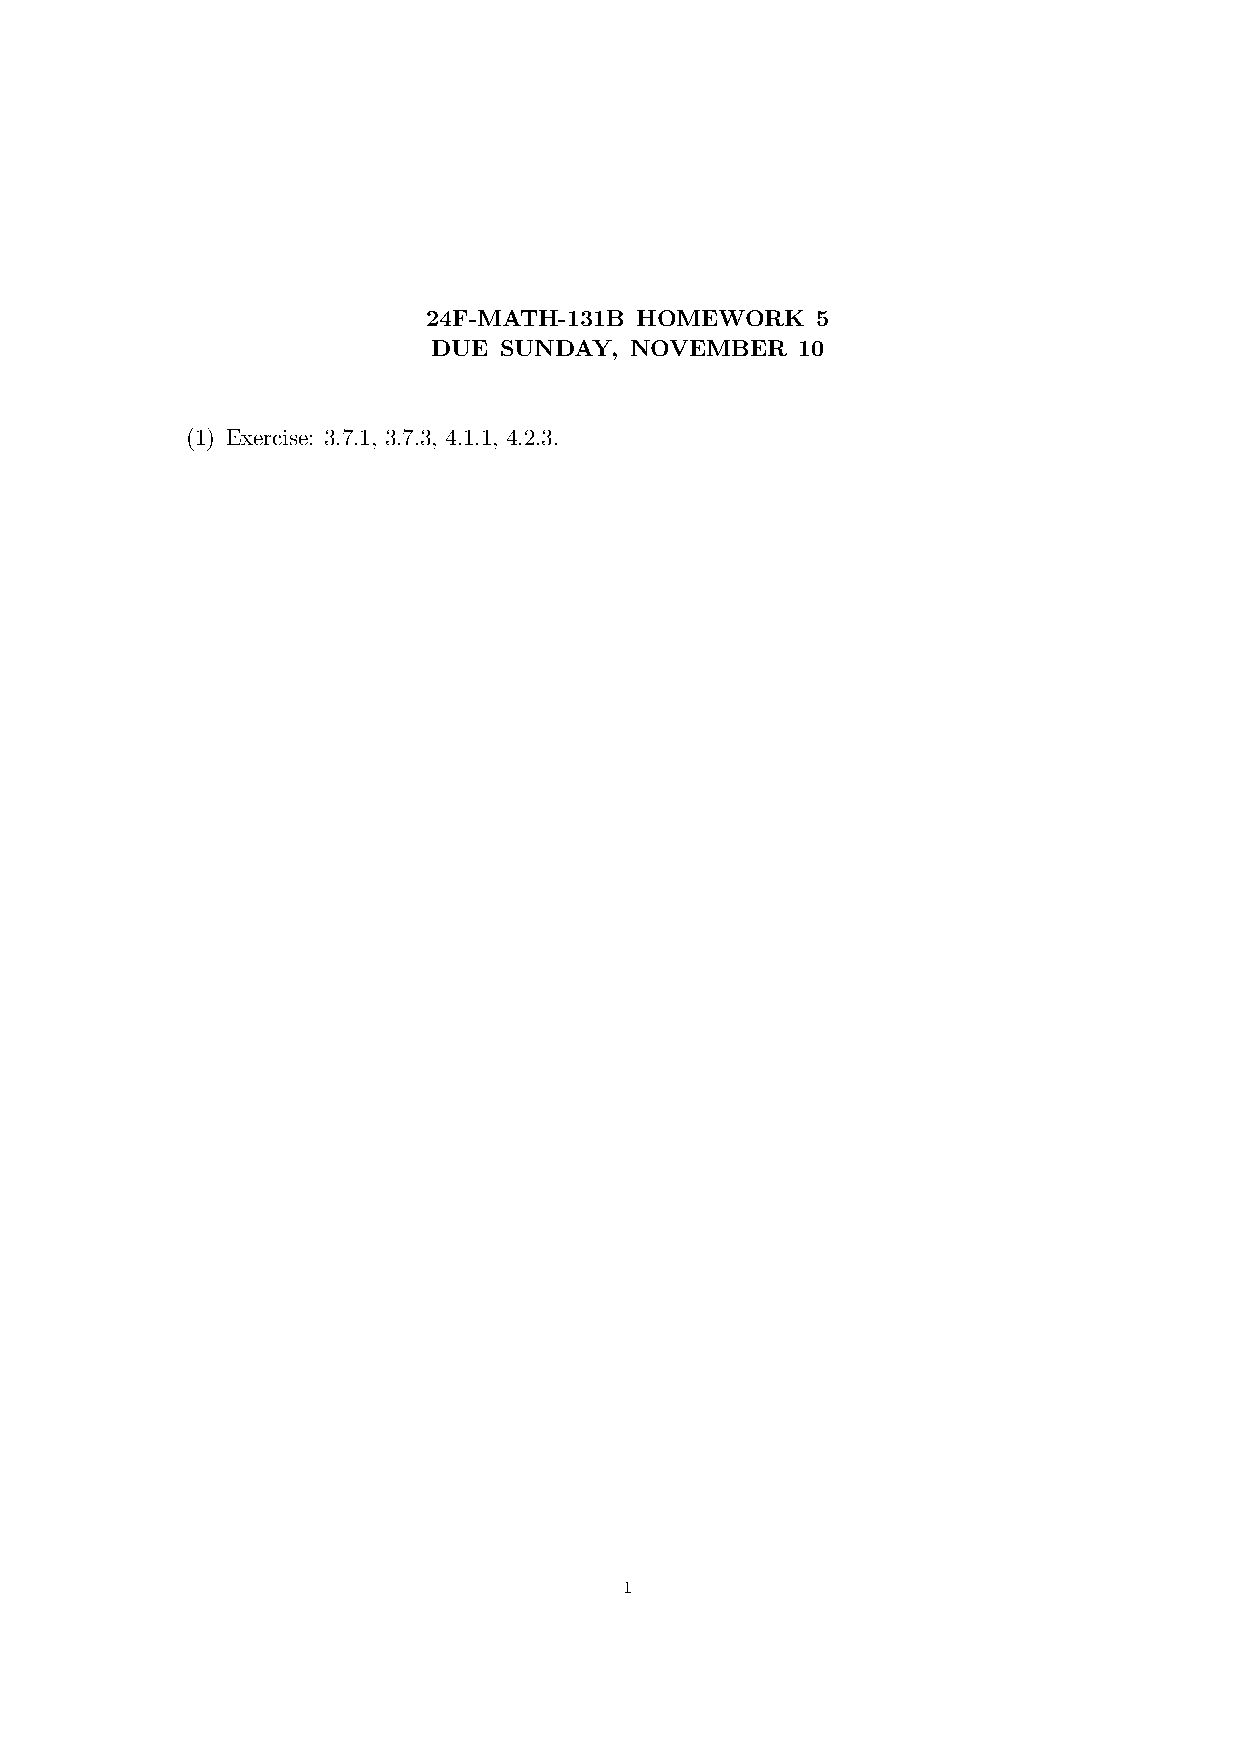
\includepdf[pages=-]{assignment.pdf}

\end{document}
